\documentclass{article}
\usepackage[UTF8]{ctex}
\usepackage[tc]{titlepic}
\usepackage{titlesec}
\usepackage{cite}
\usepackage{fancyhdr}
\usepackage{booktabs}
\usepackage{graphicx}
\usepackage{geometry}
\usepackage{enumitem}
\usepackage[section]{placeins}
\usepackage{listings}
\usepackage{xcolor}

% 设置Python代码样式
\lstset{
	language=Python,
	basicstyle=\ttfamily\small,
	keywordstyle=\color{blue},
	stringstyle=\color{red},
	commentstyle=\color{gray},
	morecomment=[s][\color{magenta}]{\^{}}{\$},
	numbers=left,
	numberstyle=\tiny\color{gray},
	stepnumber=1,
	numbersep=5pt,
	showspaces=false,
	showstringspaces=false,
	showtabs=false,
	frame=single,
	tabsize=4,
	captionpos=b,
	breaklines=true,
	breakatwhitespace=false,
	title=\lstname,
	escapeinside={(*}{*)}
}
\geometry{a4paper,scale=0.8}
\pagestyle{fancy}

\lhead{第 3 次作业\\\today}
\chead{中国科学技术大学\\深度学习导论}

\rhead{Assignment 3\\ {\CTEXoptions[today=old]\today}}
\newcommand{\upcite}[1]{\textsuperscript{\cite{#1}}}

\titleformat*{\section}{\bfseries\Large}
\titleformat*{\subsection}{\bfseries\large}

\title{\bfseries 残差卷积神经网络实现cifar-10数据集分类}
\author{陈鸿绪 \quad  少年班学院 \quad  PB21000224}
\begin{document}
	\maketitle
	\section*{\centerline{摘要}}
		本此实验任务是利用卷积神经网络实现cifar-10的数据集分类。为了得到更高的准确率,实验采取的网络基本框架为ResNet18,并采取多次保留checkpoint文件不断进行参数调整优化的方式进行训练,最终得到测试集上的准确率最高达到89.27\%(模型参数记录文件参见check\_points中的checkpoint-block-3.pth)。同时,我们通过变量消融实验探究了dropout、normalization、learning rate decay、卷积核大小、网络深度等超参数对模型性能的影响,因为实验硬件设备和时间代价过高的原因,在多次变量消融实验里,最大轮数epochs只设置为30,虽然模型大概率处于欠拟合状态,但是足够看出来这些超参数对于模型性能的影响。实验训练实验代码位于src文件夹中,代码使用说明参见README.md。\\
	
	\setcounter{section}{1}
	\section*{\centerline{一、实验原理}}
	\setcounter{subsection}{0} 
	\subsection{卷积神经网络}
	卷积神经网络(CNN)是一种广泛用于图像和视频分析的神经网络。它的工作原理是模仿人类视觉系统对视觉刺激的处理方式,通过一系列层来识别图像中的模式和特征。
	
	首先,卷积层(Convolutional Layer)使用卷积操作提取图像的局部特征,例如边缘、角点等。每个卷积核(或过滤器)在图像上滑动,生成特征映射(Feature Map),这些特征映射代表了不同特征的响应强度。
	
	接着,池化层(Pooling Layer)对特征映射进行下采样,减少数据的维度,同时保留最重要的信息。最常用的池化方法是最大池化(Max Pooling),它选择每个局部区域中的最大值作为代表。
	
	这两个层的组合可以重复多次,每次都增加卷积核的数量,以捕捉更复杂的特征。随着层的深入,网络能够识别更高级别的结构,如形状、物体部件等。
	
	最后,全连接层(Fully Connected Layer)将高维的特征映射转换为类别得分,通常在网络的最后使用softmax函数输出每个类别的概率分布。
	
	通过反向传播算法和梯度下降优化,CNN可以学习到从输入图像到输出类别的映射。这种层次化的特征提取和抽象使得CNN在图像识别、物体检测和许多其他计算机视觉任务中表现出色。
	
	\subsection{残差连接}
	残差连接(Residual Connection)是一种在深度神经网络中常用的设计技巧,尤其是用于卷积神经网络(CNN)和循环神经网络(RNN)。其核心思想是在网络中引入跳跃连接(Skip Connection),允许梯度直接传播到较早的层,从而缓解了深层网络中的梯度消失问题。
	
	在残差连接中,输入不仅传递到下一层,还直接加到后面某层的输出上。这样,网络需要学习的输出实际上是输入和层输出的差值,即“残差”。如果输入和输出的维度不同,可以通过线性变换(如使用1x1卷积)来匹配维度。
	
	没有接入残差连接的卷积神经网络模型构建的深度有限,模型过深容易导致梯度消失或梯度爆炸的情况出现。所以我们引入残差连接到神经网络中。在实验中为了提高模型性能,我们基本架构采取ResNet18。\\
	
	\setcounter{section}{2}
	\section*{\centerline{二、实验过程}}
	\setcounter{subsection}{0} 
	\subsection{构建并数据增强cifar-10数据集}
	\begin{enumerate}[label=\textbullet]
		\item 写继承于torch中Dataset的数据集类,读取cifar-10的原数据,并将其处理成图片与标签对形式。将batch1-5分为训练集,batch6与test\_batch分别作为验证集和测试集。
		\item 数据增强,我们将训练集的图片在padding为4后随机框出32×32,并对其做随机反转。计算可以得到原图数据集的三通道归一化后的平均值和方差,我们利用三个通道各自的平均值和方差对所有数据再做标准化。
	\end{enumerate}
	
	\subsection{构建残差卷积神经网络}
	ResNet18是一种经典的卷积神经网络架构,属于ResNet(Residual Network)系列,由微软研究院的Kaiming He等人在2015年提出。它的主要特点是引入了残差连接(Residual Connection)来缓解深层网络中的梯度消失问题,使得卷积神经网络可以训练得更深。
	我们使用的标准ResNet18模型架构组成如下:
	\begin{enumerate}[label=\textbullet]
	\item 初始层:通常包括一个7x7的卷积层,步长为2,后面跟着一个最大池化层(3x3,步长为2),用于减少数据的空间维度。
	\item 残差块:ResNet18包含4×2个残差块(Residual Block,这里4代表总共有四种不同的通道数目),每个块内部有两层3x3的卷积层,中间没有池化层。每个残差块内部有一个残差连接,即输入可以直接跳过卷积层,加到卷积层的输出上。这种设计允许梯度直接流过卷积层,有助于训练深层网络。
	\item 下采样层:在每个残差块的开始,使用一个步长为2的3x3卷积层进行下采样,同时增加卷积核的数量,从而减少空间尺寸并增加特征图的深度。
	\item 全局平均池化层:在所有残差块之后,使用一个全局平均池化层(Global Average Pooling)来减少特征图的维度,使其成为1x1,对应于类的数量。
	\item 全连接层:最后是一个全连接层,用于输出最终的分类得分。
	\end{enumerate}
	在本次实验中,需要探究不同超参数对网络的影响,为了不影响模型整体架构,对卷积核大小的消融实验只针对位于初始层的卷积网络;对dropout的消融实验将dropout层置于全连接层前;对网络结构的考察只针对于相同通道数的层所包含的残差块(block)个数,即每个通道数保持相同的层集合含有2个残差块(标准ResNet18)和含有3个残差块两种不同情形,实验中探索比较了两个不同深度的残差卷积网络可以达到最优分类准确率;对于Batch Normalization,我们在初始层的卷积层后考虑添加或者去除BatchNorm层。
	
	
	\subsection{调试、训练并测试网络}
	这一步主要分为两部分。第一部分是探究两种不同网络结构在测试集上的最优准确率,采取多次保留checkpoint文件不断进行学习率等参数调整优化的方式进行训练,所以这部分没有损失曲线和固定的一组参数进行分析讨论,只关注于测试集上能达到的准确率最大值。第二部分将进行变量消融实验,在固定网络架构、层数、最大轮数(epoch)、学习率等超参数基础上,这部分我们会关注特定单变量的改变以及相应的损失曲线与测试集上的准确率。\\
	\setcounter{section}{3}
	\section*{\centerline{三、关键代码讲解}}
	\setcounter{subsection}{0} 
	\subsection{数据处理代码}
	\begin{lstlisting}[language=Python, caption=数据处理代码]
	if mode == "train":
		self.data ,self.target = load_CIFAR10_data_batch(1)
		for i in range(2,5) :
			temp_data ,temp_target = load_CIFAR10_data_batch(i)
			self.data = np.concatenate([self.data,temp_data])
			self.target = np.concatenate([self.target,temp_target])
		self.transform = transforms.Compose([
			transforms.RandomCrop(32, padding=4),
			transforms.RandomHorizontalFlip(p=0.5),
			transforms.ToTensor(),
			transforms.Normalize(
				mean=(0.49139968 ,0.48215841, 0.44653091), 
				std=(0.20220212, 0.19931542, 0.20086346)
			)
		])
	else:
		if mode == "test":
			data ,target = load_CIFAR10_data_batch(6)
		elif mode == "eval":
			data ,target = load_CIFAR10_data_batch(5)
		else:
			raise NoSuchNameError("Only 'train', 'eval', 'test'")
		self.data = data
		self.target = target
		self.transform = transforms.Compose([
			transforms.ToTensor(),
			transforms.Normalize(
				mean=(0.49139968 ,0.48215841, 0.44653091), 
				std=(0.20220212, 0.19931542, 0.20086346)
			)
		])	
	self.data = self.data.reshape(-1, 3, 32, 32)
	self.data = self.data.transpose((0, 2, 3, 1))
	\end{lstlisting}
	
	 这段代码主要是将数据集的不同batch分给训练集(batch1-5)、验证集(batch6)与测试集(test\_batch),比例为5:1:1。为了增加鲁棒性,我们主要进行对训练集数据的数据增强,即将图片进行padding、随机框选以及随机反转。同时也需要将数据形式改为torch tensor的数据类型。最后根据前置计算得到图像数据集三通道归一化后分别的平均值、方差,从而进行对数据标准化操作。最后需要注意将数据张量进行合理的转置操作。\\
	
	\subsection{网络结构代码}
	
	\begin{lstlisting}[language=Python, caption=网络结构代码]
		class BLOCK(nn.Module) :
		
			def __init__(self,inplanes:int, planes:int, stride:int, downsample=None) :
			
				super(BLOCK,self).__init__() 
				self.conv1 = nn.Conv2d(inplanes,planes,3,stride,padding=1,bias=False) 
				self.bn1 = nn.BatchNorm2d(planes) 
				self.relu = nn.ReLU(inplace=True)
				self.conv2 = nn.Conv2d(planes,planes,3,stride=1,padding=1,bias=False)
				self.bn2 = nn.BatchNorm2d(planes)
				self.stride = stride
				self.downsample = downsample
			
			def forward(self,x) :
				identity = x
				out = self.conv1(x)
				out = self.bn1(out)
				out = self.relu(out)
				
				out = self.conv2(out)
				out = self.bn2(out)
				if self.downsample is not None :
					identity = self.downsample(x)
				out = out + identity
				out = self.relu(out)
				return out
		
		class ResNet(nn.Module) :
		
			def __init__(self,lays:list,num_classes:int,p: float) :
				super(ResNet,self).__init__()
				self.inplanes = 64
				# self.conv1 = nn.Conv2d(3,self.inplanes,7,stride=2,padding=3)
				self.conv1 = nn.Conv2d(3,self.inplanes,3,stride=1,padding=1)
				#稍微修改一下第一次的捲積操作,便於保留特徵
				self.bn1 = nn.BatchNorm2d(self.inplanes)
				self.relu = nn.ReLU(inplace=True)
				self.maxpool = nn.MaxPool2d(kernel_size=3,stride=1,padding=1) #後面池化操作進行刪除
				self.lay1 = self._make_lay(64,lays[0],stride=1)
				self.lay2 = self._make_lay(128,lays[1],stride=2)
				self.lay3 = self._make_lay(256,lays[2],stride=2)
				self.lay4 = self._make_lay(512,lays[3],stride=2)
				self.avgpool = nn.AdaptiveAvgPool2d((1, 1))
				self.dropout = nn.Dropout(p)
				self.fc = nn.Linear(512, num_classes)
				self.softmax = nn.Softmax(dim=1)
			
			def _make_lay(self,planes:int,num_blocks:int,stride:int) -> nn.Sequential :
				downsample = None
				if stride != 1 or self.inplanes != planes:
					downsample = nn.Sequential(nn.Conv2d(self.inplanes, planes, 1, stride=stride, bias=False), nn.BatchNorm2d(planes))
				lays = []
				lays.append(BLOCK(self.inplanes, planes, stride, downsample))
				self.inplanes = planes
				for i in range(num_blocks) :
					lays.append(BLOCK(self.inplanes,planes,stride=1))
				return nn.Sequential( *lays)
			
			def forward(self, x):
			
				x = self.conv1(x)
				x = self.bn1(x)
				x = self.relu(x)
				
				x = self.lay1(x)
				x = self.lay2(x)
				x = self.lay3(x)
				x = self.lay4(x)
				
				x = self.avgpool(x)
				x = torch.flatten(x, 1)
				x = self.dropout(x)
				x = self.fc(x)
				x = self.softmax(x)
				return x
		
	\end{lstlisting}
	
	这段代码中BLOCK用于构建残差块,每个残差块都有且只有一个残差连接,当输入与输出的通道数不同时,残差块中就会涉及到downsample,即下采样,而下采样是通过1×1卷积层实现的。ResNet类中可以看见分为五个部分,第一部分为初始层,初始层包括初始层卷积以及池化等操作。中间层按照输入输出通道数目分为4个部分,每个部分残差块的个数由\_\_init\_\_函数的lays对应的列表分量决定。输出层将做平均池化,并将结果展平后经过随机丢弃概率为p的dropout层再进入全连接层,最后进行softmax操作。
	\setcounter{section}{4}
	\section*{\centerline{四、对超参数的调试与结果分析}}
	\setcounter{subsection}{0} 
	下面我们的loss曲线表征的是训练集上的总损失,并不是平均样本损失。
	\subsection{测试不同网络深度的准确率极限}
	相同网络架构下不同网络深度必然对应着不同的拟合能力,所以如果只是单一的对网络深度调参分析、进行消融实验,如果不是为了观察欠拟合或者过拟合现象,这是不太合理的。所以我们决定考察对于不同网络深度可以到达的极限水平,由于时间成本过高,所以我们只探索了lays分别为[2, 2, 2, 2](ResNet18)以及[3, 3, 3, 3]两种得到的准确率的极限。单次训练大概率可能会因为训练阶段后段部分学习率不能和当前状态的最佳学习率耦合而导致损失不能有效下降。所以为了探索准确率的极限,我们采用多次训练保留checkpoint文件不断进行学习率等参数调整优化的方式进行训练,这样可以避免训练后阶段无效的参数更新。最后在多次训练后,得到的验证集准确率逐渐趋于稳定。对于lays为[2, 2, 2, 2](即处理相同通道数的层的残差块个数为2)的18层模型(8个残差块加上初始层卷积和输出层全连接,不包括池化、dropout等),测试集上的极限准确率为86.32\%;对于lays为[3, ,3 ,3 ,3](即处理相同通道数的层的残差块个数为3)的26层模型(12个残差块加上初始层卷积和输出层全连接,不包括池化、dropout等),测试集上的极限准确率为89.27\%。前者对应的checkpoint文件为"checkpoint-block-2",后者是"checkpoint-block-3",这是笔者训练出来在测试集上最优的准确率模型。
	
	可以发现26层深的网络准确率是高出另一个18层深的网络大约4个百分点,这说明在没有发生过拟合或者欠拟合的情况下,网络层数越深,网络表示能力就会越强。
	
	\subsection{探究不同learning rate decay对模型性能影响}
	
	\begin{table}[!ht]
		\caption{\textbf{网络超参数及结果}}%标题
		\centering%
		\begin{tabular}{ccccccccc}
			\hline
			学习率    & batch size & 最大轮数 & block个数 & decay\_rate & dropout & 最终loss & 验证集最终准确率\\ \hline
			0.001 & 512    & 30  &  2  & 1 &0 & 132.08587  & 0.7645   \\ \hline
		\end{tabular}
	\end{table}
	\clearpage
	\begin{figure}[!ht]
		\centering %居中
		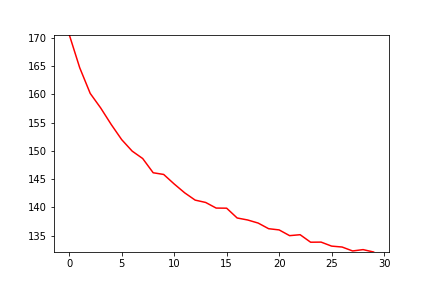
\includegraphics[scale=0.5]{runing-loss-9.png}
		\caption{训练集上损失曲线,decay\_rate为1,即学习率不会下降}
	\end{figure}
	
	\begin{table}[!ht]
		\caption{\textbf{网络超参数及结果}}%标题
		\centering%
		\begin{tabular}{ccccccccc}
			\hline
			学习率    & batch size & 最大轮数 & block个数 & decay\_rate & dropout & 最终loss & 验证集最终准确率\\ \hline
			0.001 & 512    & 30  &  2  & 0.9 &0 & 130.22897  & 0.7871   \\ \hline
		\end{tabular}
	\end{table}
	\begin{figure}[!ht]
		\centering %居中
		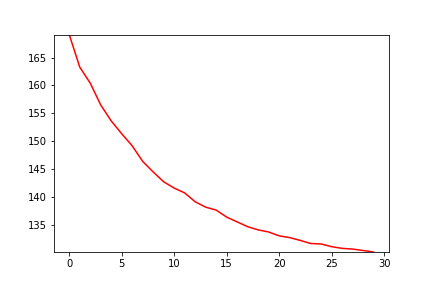
\includegraphics[scale=0.5]{runing-loss-4.png}
		\caption{训练集上损失曲线,decay\_rate为0.9}
	\end{figure}
	
	
	\begin{table}[!ht]
		\caption{\textbf{网络超参数及结果}}%标题
		\centering%
		\begin{tabular}{ccccccccc}
			\hline
			学习率    & batch size & 最大轮数 & block个数 & decay\_rate & dropout & 最终loss & 验证集最终准确率\\ \hline
			0.001 & 512    & 30  &  2  & 0.45 &0 & 154.83982  & 0.5028   \\ \hline
		\end{tabular}
	\end{table}
	\clearpage
	\begin{figure}[!ht]
	\centering %居中
	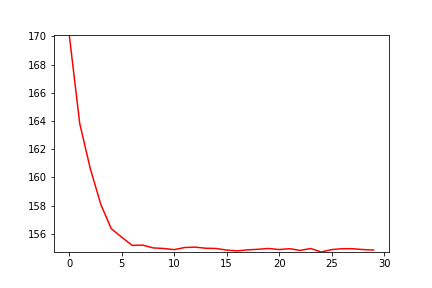
\includegraphics[scale=0.5]{runing-loss-5.png}
	\caption{训练集上损失曲线,decay\_rate为0.45}
\end{figure}

\subsection{探究不同dropout概率对模型性能影响}
\begin{table}[!ht]
	\caption{\textbf{网络超参数及结果}}%标题
	\centering%
	\begin{tabular}{ccccccccc}
		\hline
		学习率    & batch size & 最大轮数 & block个数 & decay\_rate & dropout & 最终loss & 验证集最终准确率\\ \hline
		0.001 & 512    & 30  &  2  & 0.9 &0.8 & 135.25858  & 0.7292  \\ \hline
	\end{tabular}
\end{table}


\begin{figure}[!ht]
	\centering %居中
	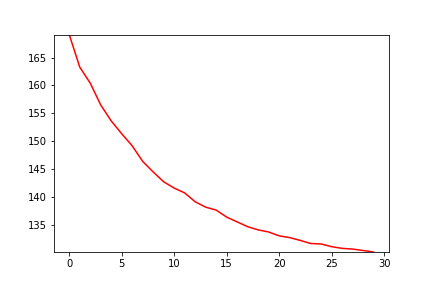
\includegraphics[scale=0.5]{runing-loss-4.png}
	\caption{训练集上损失曲线,dropout为0.8}
\end{figure}



\begin{table}[!ht]
	\caption{\textbf{网络超参数及结果}}%标题
	\centering%
	\begin{tabular}{ccccccccc}
		\hline
		学习率    & batch size & 最大轮数 & block个数 & decay\_rate & dropout & 最终loss & 验证集最终准确率\\ \hline
		0.001 & 512    & 30  &  2  & 0.9 &0.4 & 132.42525  & 0.7640   \\ \hline
	\end{tabular}
\end{table}

\clearpage

\begin{figure}[!ht]
	\centering %居中
	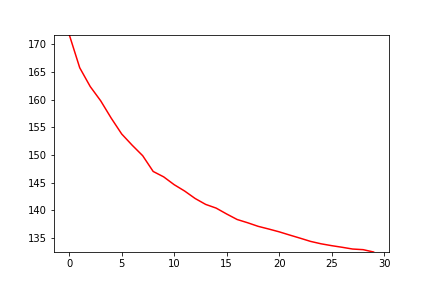
\includegraphics[scale=0.5]{runing-loss-7.png}
	\caption{训练集上损失曲线,dropout为0.4}
\end{figure}	

\begin{table}[!ht]
	\caption{\textbf{网络超参数及结果}}%标题
	\centering%
	\begin{tabular}{ccccccccc}
		\hline
		学习率    & batch size & 最大轮数 & block个数 & decay\_rate & dropout & 最终loss & 验证集最终准确率\\ \hline
		0.001 & 512    & 30  &  2  & 0.9 &0 & 130.22897  & 0.7871   \\ \hline
	\end{tabular}
\end{table}

\begin{figure}[!ht]
	\centering %居中
	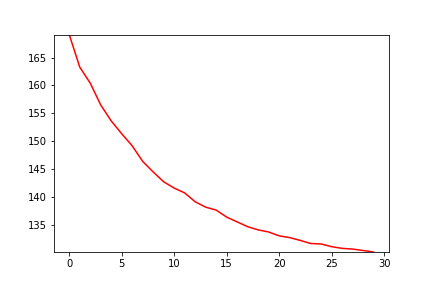
\includegraphics[scale=0.5]{runing-loss-4.png}
	\caption{训练集上损失曲线,dropout为0}
\end{figure}

\subsection{探究不同Batch Normalization对模型性能影响}

全连接层之前使用Batch Normalization(没有被注释):
\begin{table}[!ht]
	\caption{\textbf{网络超参数及结果}}%标题
	\centering%
	\begin{tabular}{ccccccccc}
		\hline
		学习率    & batch size & 最大轮数 & block个数 & decay\_rate & dropout & 最终loss & 验证集最终准确率\\ \hline
		0.001 & 512    & 30  &  2  & 0.9 &0 & 130.22897  & 0.7871   \\ \hline
	\end{tabular}
\end{table}

\clearpage
\begin{figure}[!ht]
	\centering %居中
	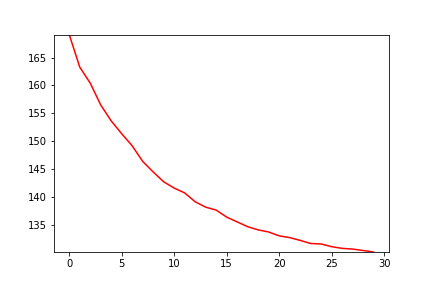
\includegraphics[scale=0.5]{runing-loss-4.png}
	\caption{训练集上损失曲线,使用了Batch Normalization}
\end{figure}

全连接层之前没有Batch Normalization(被注释):
\begin{table}[!ht]
	\caption{\textbf{网络超参数及结果}}%标题
	\centering%
	\begin{tabular}{ccccccccc}
		\hline
		学习率    & batch size & 最大轮数 & block个数 & decay\_rate & dropout & 最终loss & 验证集最终准确率\\ \hline
		0.001 & 512    & 30  &  2  & 0.9 &0 & 132.10440  & 0.7608   \\ \hline
	\end{tabular}
\end{table}

\begin{figure}[!ht]
	\centering %居中
	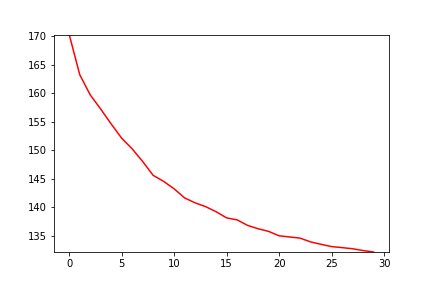
\includegraphics[scale=0.5]{runing-loss-10.png}
	\caption{训练集上损失曲线,并没有使用了Batch Normalization}
\end{figure}

\subsection{探究不同卷积核对模型性能影响}
我们只关注位于初始层的卷积层,该层可以使用两种不同的卷积核第一种(size=3, stride=1, padding=1)和第二种卷积核(size=7, stride=2, padding=3)。我们之前探究的均默认为第一种卷积核,下面我们比较两种卷积核带来的不同模型性能影响。

第一种卷积核(size=3, stride=1, padding=1):
\begin{table}[!ht]
	\caption{\textbf{网络超参数及结果}}%标题
	\centering%
	\begin{tabular}{ccccccccc}
		\hline
		学习率    & batch size & 最大轮数 & block个数 & decay\_rate & dropout & 最终loss & 验证集最终准确率\\ \hline
		0.001 & 512    & 30  &  2  & 0.9 &0 & 130.22897  & 0.7871   \\ \hline
	\end{tabular}
\end{table}

\clearpage
\begin{figure}[!ht]
	\centering %居中
	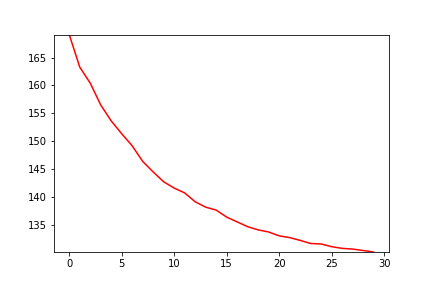
\includegraphics[scale=0.5]{runing-loss-4.png}
	\caption{训练集上损失曲线,第一种卷积核(size=3, stride=1, padding=1)}
\end{figure}

第二种卷积核(size=7, stride=2, padding=3):
\begin{table}[!ht]
	\caption{\textbf{网络超参数及结果}}%标题
	\centering%
	\begin{tabular}{ccccccccc}
		\hline
		学习率    & batch size & 最大轮数 & block个数 & decay\_rate & dropout & 最终loss & 验证集最终准确率\\ \hline
		0.001 & 512    & 30  &  2  & 0.9 &0 & 138.71478  &  0.6924  \\ \hline
	\end{tabular}
\end{table}

\begin{figure}[!ht]
	\centering %居中
	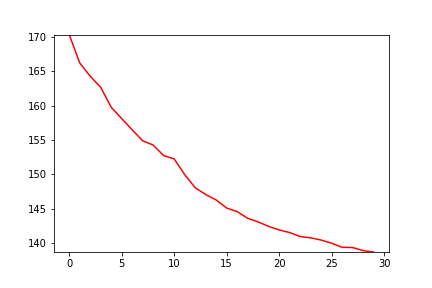
\includegraphics[scale=0.5]{runing-loss-11.png}
	\caption{训练集上损失曲线,第二种卷积核(size=7, stride=2, padding=3)}
\end{figure}

\subsection{消融实验结果分析总结}
	\begin{enumerate}[label=\textbullet]
		\item \textbf{网络深度}:从4.1节的分析就可以看出,相同类型网络的前提下,网络层数越多,网络的表示能力、提取复杂关系的能力、拟合能力就会越强。但是同样的会带来更多训练时长、推理时长的代价。在实践中需要合理设置网络深度。
		 \item \textbf{learning rate decay}:从4.2节的图1到图3和相应测试集上的准确率可以看出,learning rate decay在0.9时最终准确率是最大的,其次是取1,最后是取0.45,loss值大小则反之。在训练后段时间,模型开始出现收敛拟合的现象,这时需要步长理论上就会更小。如果学习率一直保持不变,模型就不能有效逼近梯度下降,不容易逼近更优的参数;如果学习率衰减过快,会导致模型尚未到达收敛、良好性能的阶段,就有模型参数更新缓慢。所以在learning rate decay是一个与模型参数更新较为耦合的值时,模型的参数更新就不会缓慢,同时也不会出现难以进一步优化的现象。我们可以合理猜测0.9是一个较优的learning rate decay参数。
		 \item \textbf{dropout}:观察图4到图6和相应的测试集准确率,我们发现似乎dropout似乎并没有起到作用,反而使得模型性能下降,dropout的概率越大,模型似乎性能越差。理论上,dropout作用在神经网络中中是为了增强模型的泛化性能,防止模型过拟合情形。我们在摘要中也提到了因为每一次消融实验如果都想将模型拟合较优,时间成本是巨大的,所以我们只运行了30 epoch来进行模型训练,所以模型几乎都处于欠拟合状态,所以自然地,这里dropout的作用就无法发挥,甚至会在模型欠拟合时降低模型性能。所以我们可以得出结论,在模型达到或者快要达到收敛状态时,dropout就会起到很好的防止过拟合的作用。
		 \item \textbf{Batch Normalization}:理论上,通过对每一层的输入数据进行归一化处理,可以使得每一层的输入分布更加稳定,这有助于加速神经网络的训练过程,因为模型不需要在每次迭代时都去适应输入数据分布的变化。同时还可以缓解梯度爆炸或者梯度消失的问题。单从本次实验中,其实我们只能看出来使用了Batch Normalization的模型确实优于没有使用Batch Normalization的模型。大约准确率上高了2.6\%。
		 \item \textbf{卷积核大小}:从4.5节的比较看出,两个不同大小的卷积核得到的测试集上的准确率相差非常大,小卷积核(size为3)大概比大卷积核(size为7)准确率高了约有9\%。再结合模型共有17层卷积层,然而我们只修改了第一个卷积层的卷积核大小。说明卷积核对于模型性能的影响非常大。实际上对于一层卷积层而言,卷积核越小,我们丢失的特征就越少(或者说关注的图像特征就越多),一张cifar-10图片大小为32×32,图片本身的特征就不多,如果卷积核过大,必然会造成大比例的特征丢失,进而模型性能下降严重。
	\end{enumerate}
	
	\clearpage
	\setcounter{section}{5}
	\section*{\centerline{五、选择对比实验中最佳参数并进行单次训练}}
	实际上这只是将消融实验参数组中的最优参数选出进行单次训练。具体最优准确率参见checkpoint-block-3.pth文件。
	\begin{table}[!ht]
		\caption{\textbf{网络超参数及结果}}%标题
		\centering%
		\begin{tabular}{ccccccccc}
			\hline
			学习率    & batch size & 最大轮数 & block个数 & decay\_rate & dropout & 最终loss & 测试集最终准确率\\ \hline
			0.001 & 512    & 60  &  2  & 0.9 &0 & 126.53595  & 0.8336   \\ \hline
		\end{tabular}
	\end{table}
	\begin{figure}[!ht]
		\centering %居中
		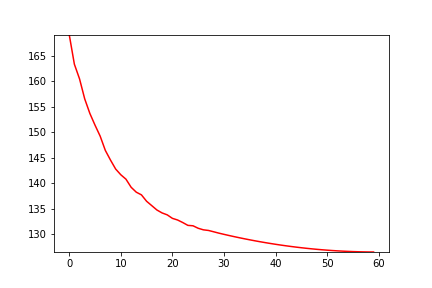
\includegraphics[scale=0.5]{runing-loss-100.png}
		\caption{训练集上损失曲线}
	\end{figure} 
\end{document}

